\documentclass[11pt]{article}
% ------------------------------------------------------------------
% Compact Dual-Timescale Latent Reasoning (CDLR)
% Plain article class so that it compiles without proprietary venue
% style files. To submit, move the body into the venue template
% (e.g. iclr20XX_conference.sty, neurips_20XX.sty, IEEEtran.cls).
% ------------------------------------------------------------------
\usepackage[margin=1in]{geometry}
\usepackage[T1]{fontenc}
\usepackage[utf8]{inputenc}
\usepackage{lmodern}
\usepackage{microtype}
\usepackage{amsmath,amssymb,amsthm}
\usepackage{booktabs}
\usepackage{tabularx}
\usepackage{multirow}
\usepackage{enumitem}
\usepackage{xcolor}
\usepackage{tikz}
\usetikzlibrary{arrows.meta,positioning,fit,backgrounds}
\usepackage[numbers,sort&compress]{natbib}
\usepackage[colorlinks=true,linkcolor=blue!50!black,citecolor=blue!50!black,urlcolor=blue!50!black]{hyperref}
\usepackage[capitalise,noabbrev]{cleveref}

\newtheorem{definition}{Definition}
\newtheorem{proposition}{Proposition}
\newtheorem{hypothesis}{Hypothesis}
\theoremstyle{remark}
\newtheorem{remark}{Remark}

\newcommand{\R}{\mathbb{R}}
\newcommand{\Sm}{\mathbf{S}}
\newcommand{\Cm}{\mathbf{C}}
\newcommand{\Hm}{\mathbf{H}}
\newcommand{\PS}{\textsuperscript{(P)}}
\newcommand{\IN}{\textsuperscript{(I)}}
\newcommand{\cdlr}{\textsc{CDLR}}

\title{\textbf{Synaptic State or KV-Cache?}\\[2pt]
\large A Unified Account of Softmax Attention, Hebbian Synaptic State, and Recurrent Latent Reasoning,\\
with a Dual-Timescale Architecture Proposal and a Matched-Compute Evaluation Protocol}

\author{Jalendar Reddy Maligireddy\\
Ph.D.\ Candidate, Information Technology, University of the Cumberlands\\
Edison, New Jersey, USA\\
\texttt{jalendarreddy97@gmail.com}}

\date{Preprint draft --- \today}

\begin{document}
\maketitle

\begin{abstract}
Softmax attention stores context as an explicit key--value cache whose size grows with sequence length; Hebbian
``synaptic'' models such as the Dragon Hatchling (BDH) store it in a fixed-size, positive, high-dimensional state
that is rewritten at every token; and recurrent latent reasoners such as BDH-CQ learn tasks from demonstrations by
writing them into such a state and then iterating in latent space. We ask a single question: \emph{when, and at what
cost, should inference-time memory be synaptic rather than a cache?} We (i) formalise all three families as
instances of one associative-memory operator with explicit write, read, forgetting, and workspace maps; (ii) show
that any single-timescale decaying state couples retention and interference, so it cannot both adapt quickly and
retain earlier episodes; (iii) specify \emph{Compact Dual-Timescale Latent Reasoning} (\cdlr), which pairs a fast
episodic Hebbian state with a slow, gated, consolidated memory bank, a halting latent workspace, a local readout
adapter, and a built-in audit trail; (iv) critically audit the empirical claims of BDH and BDH-CQ, separating
paper-stated limits from inferred gaps; and (v) specify a preregistrable, matched-parameter/token/compute
evaluation protocol that reports accuracy, memory, and latency jointly and treats negative results as first-class.
We report no large-scale results; the contribution is the framework, the analysis, the falsifiable hypotheses, and
the protocol needed to test them.
\end{abstract}

\noindent\textbf{Keywords:} attention, linear attention, fast weights, Hebbian plasticity, state-space models,
continual learning, complementary learning systems, latent reasoning, evaluation methodology.

% ==================================================================
\section{Introduction}
\label{sec:intro}

The Transformer \citep{vaswani2017attention} replaced recurrence with attention ``dispensing with recurrence and
convolutions entirely'' (\citealp{vaswani2017attention}, Abstract) and accepted an $O(T^2 d)$ per-layer cost in
sequence length $T$ in exchange for constant path length and full parallelism (\citealp{vaswani2017attention},
\S4, Table~1). At inference time this design keeps every past key and value: the context is \emph{stored},
not \emph{learned}. Two recent papers from the Pathway group challenge this choice from the opposite end.
\emph{The Dragon Hatchling} (BDH; \citealp{kosowski2025bdh}) argues that inference-time working memory can rely
``entirely on synaptic plasticity with Hebbian learning'' (Abstract), in a state of size $n\times d$ per layer that
does not grow with context (\S3, Eq.~5), and reports parity with GPT-2-style baselines from 10M to 1B parameters on
Europarl translation (\S4.2, Fig.~7). \emph{BDH-CQ} \citep{engdahl2026bdhcq} builds a reasoning system in which
demonstrations update a recurrent memory and a query is solved by iterating in latent space without verbal chain of
thought (\S3.2--3.3, Eqs.~1--4), reporting 29.5\% pass@2 on the public ARC-AGI-1 evaluation at a computed
\$0.00070 per task (\S5, Table~1).

These are strong and interesting claims. They also leave open the question that matters for the next
architecture class: \textbf{is a fixed-size synaptic state a better inference-time memory than a KV-cache, and
under what accounting?} Four observations motivate this paper.
\begin{enumerate}[leftmargin=*,itemsep=1pt]
\item The three families are usually described in incompatible vocabularies (operators, synapses, recurrent
memory), which hides what is actually different: what is written, how it is forgotten, and how it is read.
\item ``Bounded'' is not ``small''. A state of $n\times d$ with $n=32{,}768$ and $d=256$ per layer
(\citealp{kosowski2025bdh}, \S4.1) is larger than a 768-wide Transformer's KV-cache until several thousand tokens
(\cref{sec:formal}). Memory claims therefore need explicit byte accounting.
\item A single decaying state cannot both adapt to a new task and keep an old one: retention and interference are
the same quantity (\cref{prop:coupling}). BDH's own merged-model language mixing
(\citealp{kosowski2025bdh}, \S7.1) and the near-total forgetting of our own preliminary probes
(\cref{app:probes}) are consistent with this. Complementary learning systems theory
\citep{mcclelland1995cls,kumaran2016cls} and synaptic consolidation models \citep{fusi2005cascade,benna2016consolidation}
suggest the remedy: a second, slower timescale.
\item The evidence base is narrow: one corpus family and a GPT-2-style baseline for BDH
(\citealp{kosowski2025bdh}, \S4.2, App.~B.2), one benchmark family and proprietary internals for BDH-CQ
(\citealp{engdahl2026bdhcq}, \S3.3, \S4.1). Neither compares against modern linear-recurrent models such as
Mamba \citep{gu2023mamba}, RetNet \citep{sun2023retnet}, xLSTM \citep{beck2024xlstm}, Gated/Delta linear attention
\citep{yang2024gla,yang2024deltanet,yang2025gateddelta} or test-time-memory models such as Titans
\citep{behrouz2025titans} at matched compute.
\end{enumerate}

\paragraph{Contributions.} The contributions below do not depend on any experiment we ran.
\begin{enumerate}[label=\textbf{C\arabic*.},leftmargin=*,itemsep=2pt]
\item \textbf{Unified formalisation (\cref{sec:formal}).} We define an \emph{associative-memory operator}
$(\mathcal{M},\omega,\rho,\lambda,\kappa,\mathcal{F})$ and place softmax attention, linear attention and SSMs,
BDH-GPU, graph-form BDH, BDH-CQ, and \cdlr{} in it, with matching byte and FLOP accounting.
\item \textbf{A plasticity--stability result for single-timescale states (\cref{prop:coupling}).} For any state with
data-independent exponential forgetting, the retention of an old episode and its interference with a new one
are the same function of lag, so no choice of decay can get both. We discuss when input-dependent gating weakens
this.
\item \textbf{The \cdlr{} architecture class (\cref{sec:method}).} A fast episodic Hebbian state $\Sm$, a slow
gated consolidated bank $\Cm$, a halting latent workspace, a local (no-BPTT) readout adapter, and an audit
interface that can certify ``no parameter updates at inference''. We state four falsifiable hypotheses (H1--H4).
\item \textbf{A critical audit of BDH and BDH-CQ (\cref{sec:critique}).} Every claim is tied to a section or
table, and we separate paper-stated limitations\PS{} from gaps we infer\IN. Among the inferred gaps are an
unreconciled cost basis in BDH-CQ and a 1B--600B scaling statement that no reported data supports.
\item \textbf{A matched-compute evaluation protocol (\cref{sec:protocol}).} Five experiment tracks (language
modelling bakeoff beyond Europarl; associative-recall capacity and length generalisation testing BDH Claim~7; an
ablation ladder isolating Hebbian and dual-timescale effects from plain linear attention; continual streams;
black-box or labelled-reimplementation latent reasoning). Results are reported as accuracy $\times$ memory
$\times$ latency Pareto fronts, with a preregistration and negative-results policy.
\end{enumerate}

\paragraph{Scope and honesty statement.} This is a framework, analysis, and protocol paper. We do \emph{not}
claim ARC-AGI parity with BDH-CQ, scaling to hundreds of billions of parameters, or a solution to the
no-backpropagation-through-time gap of \citet[\S7.2]{kosowski2025bdh}. The only numbers we report from our own
code are small CPU probes, kept to \cref{app:probes} and labelled as such.

% ==================================================================
\section{Background and Related Work}
\label{sec:related}

\paragraph{Softmax attention.} Scaled dot-product attention computes
$\mathrm{softmax}(QK^\top/\sqrt{d_k})V$ (\citealp{vaswani2017attention}, Eq.~1), with $h=8$ heads of
$d_k=d_v=64$ in the base model (\S3.2.2). The authors note the $O(T^2d)$ cost, propose restricted attention for
long inputs, and list less sequential generation as future work (\S4, \S7). Later work made exact attention
IO-efficient \citep{dao2022flashattention} and added relative positions \citep{su2024roformer,press2022alibi} and
segment recurrence \citep{dai2019transformerxl}. The inference-time KV-cache, which \citet[Table~3]{kosowski2025bdh}
describes as ``not localized at neurons'', grows linearly in $T$.

\paragraph{Linear attention, fast weights, and SSMs.} Replacing the softmax kernel with a feature map $\phi$ turns
attention into a recurrence on the matrix $\sum_\tau \phi(k_\tau)v_\tau^\top$ \citep{katharopoulos2020transformers,
choromanski2021performer}. \citet{schlag2021linear} showed that this is a fast-weight programmer
\citep{ba2016fastweights} and introduced a delta-rule update. Gated, decayed, and selective variants include RetNet
\citep{sun2023retnet}, GLA \citep{yang2024gla}, Mamba \citep{gu2023mamba}, Mamba-2 with its state-space duality
\citep{dao2024ssd}, xLSTM \citep{beck2024xlstm}, DeltaNet \citep{yang2024deltanet}, and Gated DeltaNet
\citep{yang2025gateddelta}. Test-time-training layers \citep{sun2024ttt}, Titans \citep{behrouz2025titans}, and
the test-time-regression view \citep{wang2025testtimeregression} read all of these as online optimisation of an
associative memory. Our formalisation (\cref{sec:formal}) follows this line. What we add is to place BDH's
positive high-dimensional neuron state and BDH-CQ's latent workspace in the same frame, and to make a
\emph{consolidation} map $\kappa$ explicit. Prior unifications leave $\kappa$ implicit or absent. Fixed-state models
are known to trail attention on associative recall and copying \citep{arora2023zoology,jelassi2024repeat}. Any
claim for synaptic memory must therefore be tested on exactly those tasks (\cref{sec:protocol}, E2).
\citet{ahn2024linear} use a shallow linear Transformer to reproduce Transformer \emph{optimisation} phenomena
(Adam--SGD gap, heavy-tailed gradient noise); it is an analysis proxy, not an efficient-attention architecture, and
its protocol has not been applied to BDH-GPU.

\paragraph{BDH.} BDH models a language model as local graph dynamics among $n$ neuron particles with Hebbian
synapse reweighting (\citealp{kosowski2025bdh}, \S2, Table~1). Its tensor form BDH-GPU$(n,d)$ has
$(3+o(1))nd$ parameters, with $E\in\R^{d\times n}$ and $D_x,D_y\in\R^{n\times d}$, positive ReLU activations, and
linear attention in neuron dimension $n$ (\S3, Def.~4, Eq.~4). It scales in $n$ with $d=256$ fixed
(App.~B.2, Table~5), and the authors report about 5\% non-zero activations (\S4.1), emergent modular scale-free
structure (\S5), and monosemantic synapses (\S6.3). Claim~7 (\S6.1, App.~C.2) states that linear attention in
$\R^n$ can separate $\tilde O(n)$ facts under non-adversarial keys and $\tilde\Omega(\sqrt n)$ without assumptions.

\paragraph{BDH-CQ and latent reasoning.} BDH-CQ writes demonstrations into $\Sm_t=U_\theta(\Sm_{t-1},D_t)$ with
fixed $\theta$, initialises a workspace $\Hm_0=E_\theta(x^*,\Sm_K)$, iterates $\Hm_{r+1}=F_\theta(\Hm_r,\Sm_K)$, and
decodes $\hat y=G_\theta(\Hm_R)$ (\citealp{engdahl2026bdhcq}, \S3.2--3.3, Eqs.~1--4). Related latent and recurrent
depth approaches include Universal Transformers \citep{dehghani2019universal}, adaptive computation time
\citep{graves2016act}, Coconut \citep{hao2024coconut}, and recurrent-depth scaling \citep{geiping2025recurrent},
in contrast to verbal chain of thought \citep{wei2022cot}. On ARC \citep{chollet2019measure}, HRM
\citep{wang2025hrm} and TRM \citep{jolicoeur2025trm} are recurrent solvers; BDH-CQ distinguishes itself by not using
task identities or evaluation demonstrations in training (\citealp{engdahl2026bdhcq}, \S1--2).

\paragraph{Continual learning and complementary learning systems.} Sequential training causes catastrophic
interference \citep{mccloskey1989catastrophic,french1999catastrophic}. Remedies include regularisation
\citep{kirkpatrick2017ewc,zenke2017si}, episodic memory and replay \citep{lopezpaz2017gem,rolnick2019replay}, and
episodic control \citep{pritzel2017nec}. Deep networks also lose plasticity under long streams
\citep{dohare2024loss}. Complementary learning systems (CLS) theory holds that a fast hippocampal system stores
episodes and a slow neocortical system consolidates them through interleaved replay
\citep{mcclelland1995cls,kumaran2016cls}. Cascade and multi-timescale synapse models show that coupling fast and
slow variables extends memory lifetime far beyond a single exponential \citep{fusi2005cascade,benna2016consolidation}.
Hebbian and three-factor rules \citep{hebb1949organization,oja1982simplified,gerstner2018eligibility} and
differentiable plasticity \citep{miconi2018differentiable} supply the local update rules we use. \cdlr{} differs in where it puts the slow timescale: at
\emph{inference time, across episodes}, with explicit gating, a fixed byte budget, and an audit trail.

% ==================================================================
\section{A Unified Formalisation of Inference-Time Memory}
\label{sec:formal}

\paragraph{Notation.} $T$ is the sequence length (tokens) and $n$ the BDH neuron count. These two axes are often
both written ``$n$'' in the literature (\citealp{vaswani2017attention}, Table~1, vs.\ \citealp{kosowski2025bdh},
\S3), and conflating them produces misleading complexity comparisons. We write $d$ for the low-rank/model width,
$L$ for layers, and $b$ for bytes per stored scalar.

\begin{definition}[Associative-memory operator]
\label{def:amo}
An inference-time memory layer is a tuple $(\mathcal{M},\omega,\rho,\lambda,\kappa,\mathcal{F})$: a state space
$\mathcal{M}$; a \emph{write} $\omega:\mathcal{M}\times\mathcal{X}\to\mathcal{M}$ applied per input; a \emph{read}
$\rho:\mathcal{M}\times\mathcal{Q}\to\R^{d_v}$; a \emph{forgetting} map $\lambda$ (decay, gating, or eviction); an
optional \emph{consolidation} map $\kappa:\mathcal{M}\times\mathcal{B}\to\mathcal{B}$ into a slower store
$\mathcal{B}$; and an optional \emph{workspace} $\mathcal{F}$ that iterates reads before emitting output. Slow
parameters $\theta$ are fixed at inference unless stated.
\end{definition}

\Cref{tab:unified} instantiates the definition. The rows differ in three places: (a)~whether $\mathcal{M}$ grows
with $T$; (b)~whether keys live in a low signed space ($d_k=64$) or a high positive sparse space ($n\sim10^4$--$10^6$);
(c)~whether $\kappa$ and $\mathcal{F}$ exist.

\begin{table}[t]
\centering
\footnotesize
\setlength{\tabcolsep}{3pt}
\caption{Inference-time memory as an associative-memory operator (\cref{def:amo}). Entries for prior work cite
the source; ``n.d.''\ = not disclosed. $\phi$ is a feature map, $\odot$ the Hadamard product, $U$ a decay/rotation
operator, $G_s$ a sparse synapse mask.}
\label{tab:unified}
\begin{tabularx}{\linewidth}{@{}>{\raggedright\arraybackslash}p{2.9cm}>{\raggedright\arraybackslash}X>{\raggedright\arraybackslash}p{3.3cm}>{\raggedright\arraybackslash}p{2.2cm}c c@{}}
\toprule
Model & State $\mathcal{M}$ and write $\omega$ & Read $\rho$ & Forget $\lambda$ & $\kappa$ & $\mathcal{F}$\\
\midrule
Softmax attn.\ \citep{vaswani2017attention} & append $(k_t,v_t)$; size $2Td$ & $\mathrm{softmax}(q^\top K/\sqrt{d_k})V$ & none (window) & -- & -- \\
Linear attn.\ \citep{katharopoulos2020transformers} & $\Sm\!\leftarrow\!\Sm+\phi(k)v^\top$; $d_\phi\times d$ & $\phi(q)^\top\Sm/\phi(q)^\top z$ & none & -- & -- \\
RetNet/GLA/Mamba-2 \citep{sun2023retnet,yang2024gla,dao2024ssd} & $\Sm\!\leftarrow\!\Lambda_t\Sm+k v^\top$ & $q^\top\Sm$ & fixed or input-gated & -- & -- \\
DeltaNet \citep{yang2024deltanet,yang2025gateddelta} & $\Sm\!\leftarrow\!\Sm+\beta k(v-\Sm^\top k)^\top$ & $q^\top\Sm$ & overwrite (+gate) & -- & -- \\
Titans \citep{behrouz2025titans} & MLP weights by surprise gradient & MLP$(q)$ & weight decay & -- & -- \\
BDH-GPU \citep[Eq.~4--5]{kosowski2025bdh} & $\rho\!\leftarrow\!(\rho+v^*x^\top)U$; $n\times d$/layer, $x\!\ge\!0$ sparse & $\rho\,x_t$ (positive $x_t\in\R^n$) & RoPE/ALiBi-like $U$ (\S2.4, \S6.1) & -- & -- \\
BDH graph \citep[Eq.~6]{kosowski2025bdh} & $\sigma\!\leftarrow\!\sigma+(yx^\top\!\odot G_s)U$ on edges & local E/I dynamics & $U$ & -- & -- \\
BDH-CQ \citep[Eqs.~1--4]{engdahl2026bdhcq} & $\Sm_t=U_\theta(\Sm_{t-1},D_t)$, n.d. & via $E_\theta,F_\theta$, n.d. & n.d. & -- & $R$ loops \\
\textbf{\cdlr{} (ours)} & fast $\Sm$ (Hebbian/delta) + slow bank $\Cm$ & normalised read of $\Sm$ and gated $\Cm$ & decay on $\Sm$; gated on $\Cm$ & \checkmark & halting $R$ \\
\bottomrule
\end{tabularx}
\end{table}

\paragraph{Attention as operator vs.\ synaptic state vs.\ recurrent latent memory.}
Softmax attention is a \emph{nonparametric} memory: the read is a kernel smoother over stored pairs, and nothing
is learned at inference. Linear attention, SSMs and BDH-GPU are \emph{parametric} memories: the read is a linear
map whose matrix is \emph{learned online} by a Hebbian (outer-product) or delta (error-correcting) rule. The
fast-weight view of \citet{schlag2021linear} makes this exact. BDH-GPU adds two biases: keys/queries are positive
and sparse in a high dimension $n\gg d$, and the per-model weights are shared across layers
(\citealp{kosowski2025bdh}, \S4.1). BDH-CQ adds a third element, a \emph{workspace} that re-reads a fixed
$\Sm_K$ for $R$ steps (\citealp{engdahl2026bdhcq}, Eq.~3). Iterative computation is thereby separated from token
emission. In \cref{def:amo} this is $\mathcal{F}$.

\paragraph{Byte accounting.} Per layer and per sequence, a softmax KV-cache stores $2Td_{\text{model}}b$ bytes,
growing in $T$. BDH-GPU stores $n d\, b$ bytes regardless of $T$ (\citealp{kosowski2025bdh}, Eq.~5). The two are
equal at
\begin{equation}
T^\star=\frac{n\,d}{2\,d_{\text{model}}}.
\label{eq:crossover}
\end{equation}
For the 25M BDH-GPU configuration ($n=32{,}768$, $d=256$; \citealp{kosowski2025bdh}, \S4.1) against a
$d_{\text{model}}=768$ Transformer, $T^\star\approx5{,}461$ tokens per layer\IN. Below $T^\star$ the bounded state
is the \emph{larger} memory. This is consistent with, and independent of, the paper's FLOP crossover of about 4096
tokens at $d=256$ (\S4.2). Constant memory pays off only for long contexts or many concurrent episodes, and fair
comparisons must report bytes at several $T$ rather than asymptotic class alone (\cref{sec:protocol}).

\paragraph{Capacity.} For a linear associative state with $n$-dimensional keys, interference between stored
items grows with key overlap. BDH Claim~7 (\S6.1; App.~C.2) gives $\tilde O(n)$ separable facts for
non-adversarial keys and $\tilde\Omega(\sqrt n)$ in the worst case. To our knowledge it has not been measured
against recall benchmarks \citep{arora2023zoology}. We turn this into hypothesis H1 (\cref{sec:method}) and
experiment E2.

\subsection{Single-timescale states couple retention and interference}
\label{sec:coupling}

Consider a linear state with data-independent forgetting, $\Sm_t=\lambda\Sm_{t-1}+u_t$, $0<\lambda<1$, where $u_t$
is the write at step $t$ (Hebbian $\phi(k_t)v_t^\top$ or similar). Let a stream switch at time $t_0$ from task $A$
(writes $u^A_t$) to task $B$ (writes $u^B_t$), with both stationary in mean, $\mathbb{E}u^A=\bar u^A$,
$\mathbb{E}u^B=\bar u^B$.

\begin{proposition}[Retention--interference coupling]
\label{prop:coupling}
At lag $\Delta\ge0$ after the switch, in expectation and in the stationary limit before $t_0$,
\[
\mathbb{E}\,\Sm_{t_0+\Delta}=\tfrac{1}{1-\lambda}\big(\lambda^{\Delta}\,\bar u^A+(1-\lambda^{\Delta})\,\bar u^B\big).
\]
The normalised weight of task $A$, $\alpha(\Delta)=\lambda^\Delta$, is simultaneously (i)~the \emph{retention} of
$A$ (the signal available for a later $A$-query) and (ii)~the \emph{interference} of $A$ with $B$-queries. Define
retention horizon $H_{\mathrm{ret}}(\varepsilon)=\min\{\Delta:\alpha(\Delta)\le\varepsilon\}$ and adaptation horizon
$H_{\mathrm{ad}}(\delta)=\min\{\Delta:\alpha(\Delta)\le\delta\}$. For any $\lambda$,
$H_{\mathrm{ret}}(\varepsilon)/H_{\mathrm{ad}}(\delta)\to\log\varepsilon/\log\delta$, independent of $\lambda$.
In particular, if $A$ must stay retrievable ($\alpha\ge\varepsilon$) and $B$ must be uncontaminated
($\alpha\le\delta$) at the same lag, with $\varepsilon>\delta$, no $\lambda$ satisfies both.
\end{proposition}
\begin{proof}[Proof sketch]
Unroll the recursion: $\Sm_{t_0+\Delta}=\lambda^\Delta\Sm_{t_0}+\sum_{j=1}^{\Delta}\lambda^{\Delta-j}u^B_{t_0+j}$.
In the stationary limit, $\mathbb{E}\Sm_{t_0}=\bar u^A/(1-\lambda)$, and $\sum_{j}\lambda^{\Delta-j}=(1-\lambda^\Delta)/(1-\lambda)$.
Both horizons solve $\lambda^\Delta=c$, so $\Delta=\log c/\log\lambda$; their ratio does not depend on $\lambda$.
Requiring $\lambda^\Delta\ge\varepsilon>\delta\ge\lambda^\Delta$ is a contradiction.
\end{proof}

\begin{remark}[What the proposition does and does not say]
It is a statement about one shared, linearly superposed state. It does not rule out good continual behaviour for
(a)~input-dependent gates ($\lambda_t$ in Mamba/GLA/Gated DeltaNet), which can freeze the state but then also stop
adapting, unless a gate learns \emph{when} a new task starts (task-boundary inference); (b)~delta rules, which
remove interference along overwritten keys but also erase the overwritten association; (c)~high-dimensional sparse
keys, which reduce overlap between $\bar u^A$ and $\bar u^B$ so that $A$ and $B$ coexist. Case (c) is BDH's
implicit bet. It holds only while tasks occupy near-disjoint neurons, which the language mixing of
\citet[\S7.1]{kosowski2025bdh} suggests is not guaranteed. The cascade models of \citet{fusi2005cascade} and
\citet{benna2016consolidation} escape the coupling by adding variables with different time constants. This is the
design principle behind \cdlr.
\end{remark}

% ==================================================================
\section{Compact Dual-Timescale Latent Reasoning (\cdlr)}

\noindent\textit{Specification pending empirical confirmation.}
Until E3 (including the byte-transfer control) and E4 land, \cdlr{} should be read as a design class and evaluation target, not a demonstrated method.
\label{sec:method}

\cdlr{} is an architecture \emph{class}, specified by the operator of \cref{def:amo} with both $\kappa$ and
$\mathcal{F}$ present and a hard byte budget. \Cref{fig:cdlr} gives the data flow.

\begin{figure}[t]
\centering
\resizebox{\linewidth}{!}{%
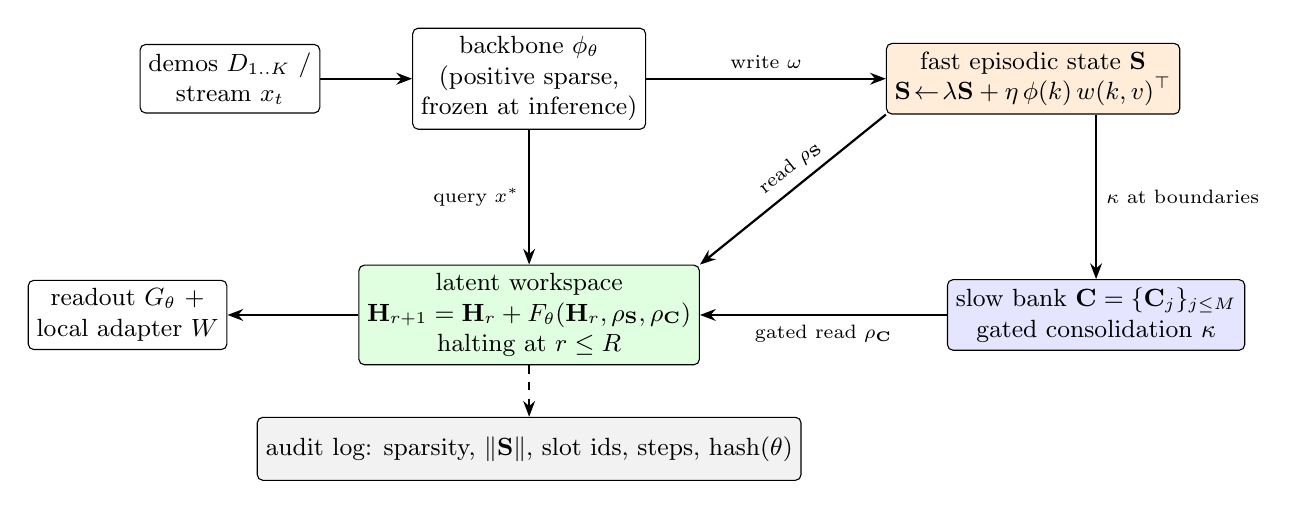
\begin{tikzpicture}[
  box/.style={draw,rounded corners=2pt,align=center,font=\small,minimum height=8mm,inner sep=3pt},
  fast/.style={box,fill=orange!15},
  slow/.style={box,fill=blue!10},
  ws/.style={box,fill=green!12},
  arr/.style={-{Stealth[length=2mm]},thick}]
\node[box] (in) at (-0.6,0) {demos $D_{1..K}$ /\\ stream $x_t$};
\node[box] (phi) at (3.2,0) {backbone $\phi_\theta$\\(positive sparse,\\ frozen at inference)};
\node[fast] (S) at (9.6,0) {fast episodic state $\Sm$\\$\Sm\!\leftarrow\!\lambda\Sm+\eta\,\phi(k)\,w(k,v)^\top$};
\node[ws] (H) at (3.2,-3.0) {latent workspace\\$\Hm_{r+1}=\Hm_r+F_\theta(\Hm_r,\rho_\Sm,\rho_\Cm)$\\halting at $r\le R$};
\node[slow] (C) at (10.4,-3.0) {slow bank $\Cm=\{\Cm_j\}_{j\le M}$\\gated consolidation $\kappa$};
\node[box] (G) at (-1.9,-3.0) {readout $G_\theta$ +\\local adapter $W$};
\node[box,fill=gray!10] (A) at (3.2,-4.7) {audit log: sparsity, $\|\Sm\|$, slot ids, steps, $\mathrm{hash}(\theta)$};
\draw[arr] (in) -- (phi);
\draw[arr] (phi) -- node[above,font=\scriptsize]{write $\omega$} (S);
\draw[arr] (S.south -| C.north) -- node[right,font=\scriptsize]{$\kappa$ at boundaries} (C.north);
\draw[arr] (S.south west) -- node[pos=0.45,above,sloped,font=\scriptsize]{read $\rho_\Sm$} (H.north east);
\draw[arr] (C) -- node[below,font=\scriptsize]{gated read $\rho_\Cm$} (H);
\draw[arr] (phi) -- node[left,font=\scriptsize]{query $x^*$} (H);
\draw[arr] (H) -- (G);
\draw[arr,dashed] (H) -- (A);
\end{tikzpicture}}
\caption{\cdlr{} data flow. Orange: fast timescale (within episode, decays). Blue: slow timescale (across episodes,
gated, never overwritten by an unmatched task). Green: latent workspace. Slow parameters $\theta$ are frozen at
inference; only $\Sm$, $\Cm$ and the optional readout adapter change, and the audit log records every change.}
\label{fig:cdlr}
\end{figure}

\paragraph{Backbone.} $\phi_\theta:\mathcal{X}\to\R^n_{\ge0}$ maps inputs to positive, sparse,
high-dimensional codes. The reference instantiation is a BDH-GPU stack (\citealp{kosowski2025bdh}, Def.~4) with
k-winners-take-all sparsification and $\ell_2$ normalisation. A Transformer or SSM backbone with a positive
projection head is a valid control, which lets the protocol separate ``BDH backbone'' effects from ``memory
architecture'' effects.

\paragraph{Fast episodic state $\Sm$.} $\Sm\in\R^{n\times d_v}$ with normaliser $z\in\R^n$:
\begin{equation}
\Sm\leftarrow\lambda\Sm+\eta\,\phi(k)\,w_\theta(k,v)^\top,\qquad z\leftarrow\lambda z+\eta\,\phi(k),\qquad
\rho_\Sm(q)=\frac{\phi(q)^\top\Sm}{\phi(q)^\top z+\epsilon}.
\label{eq:fast}
\end{equation}
$\eta=\mathrm{softplus}(\cdot)$ and $\lambda=\mathrm{sigmoid}(\cdot)$ are slow parameters. A delta-rule variant
$\Sm\leftarrow\lambda\Sm+\eta\,\phi(k)(w-\Sm^\top\phi(k))^\top$ \citep{schlag2021linear,yang2024deltanet} is a
first-class ablation, because it changes the capacity regime of H1.

\paragraph{Slow consolidated bank $\Cm$ and consolidation $\kappa$.} $\Cm=\{(\Cm_j,\mathbf{k}_j)\}_{j=1}^{M}$ holds
at most $M$ slots, each a matrix of the shape of $\Sm$ (or a rank-$r$ factorisation), with a summary key
$\mathbf{k}_j$. A small reservoir buffer $\mathcal{R}$ of past codes supports replay, as in CLS
\citep{mcclelland1995cls}. At a consolidation event (an episode boundary, or a novelty trigger when the read error
of $\Sm$ exceeds a threshold), we form a candidate
$\hat\Cm=\mathrm{unit}\big(\tfrac12\Sm+\tfrac12\,\Pi(\mathcal{R})\big)$, where $\Pi$ computes class- or
key-conditioned means of replayed codes. Let $j^\star=\arg\max_j\cos(\hat\Cm,\Cm_j)$. Then
\begin{equation}
\kappa:\;\begin{cases}
\Cm_{j^\star}\leftarrow(1-\beta)\Cm_{j^\star}+\beta\hat\Cm & \text{if }\cos(\hat\Cm,\Cm_{j^\star})\ge\tau,\\
\text{allocate a new slot (evict least-used if }|\Cm|=M) & \text{otherwise.}
\end{cases}
\label{eq:consolidate}
\end{equation}
Reads from $\Cm$ are gated: $g_j=\mathrm{softmax}_j(\gamma\cdot s_j)$, where $s_j$ is either key similarity
$\cos(\mathbf{k}_j,\bar\phi_{\text{ctx}})$ (unsupervised) or the fit of $\Cm_j$ to a small labelled support set
(supervised; this leaks task information and must be reported as such). The term is omitted when
$\max_j s_j<\tau_{\text{gate}}$. Because $\Cm_j$ is only written when matched, task $A$'s slot is not diluted by
task $B$'s writes, which breaks the coupling of \cref{prop:coupling} at the cost of $M$ extra states and a
task-boundary or novelty signal.

\paragraph{Latent workspace.} Following BDH-CQ's public equations (\citealp{engdahl2026bdhcq}, Eqs.~2--4), but
with our own open choices for every function:
\begin{align}
\Hm_0&=E_\theta\big(x^*,\rho_\Sm(\phi(x^*)),\textstyle\sum_jg_j\rho_{\Cm_j}(\phi(x^*))\big),\\
\Hm_{r+1}&=\Hm_r+F_\theta\big([\Hm_r;\rho_\Sm(\kappa_k(W_q\Hm_r))]\big),\quad r<R,\\
\hat y&=G_\theta(\Hm_{r^\star}),\quad r^\star=\min\{r:\max\mathrm{softmax}(G_\theta(\Hm_r))\ge c\}\wedge R,
\end{align}
where $\kappa_k$ is k-WTA and $c$ a confidence threshold for halting, as in ACT \citep{graves2016act}. Every
re-read uses the same $\Sm$, so the workspace adds compute but no memory that grows with $R$.

\paragraph{Local adapter.} An optional readout $W\phi+b$ adapts online by a three-factor rule
\citep{gerstner2018eligibility}: $e_t=\gamma e_{t-1}+\phi_t$, $W\mathrel{+}=\eta_W(y_t-p_t)e_t^\top$. Nothing flows
into the backbone or back through time. For a linear head with $\gamma=0$ this coincides with the cross-entropy
gradient of that head. Its locality lies in what it does \emph{not} touch, and we do not claim it closes the
no-BPTT gap of \citet[\S7.2]{kosowski2025bdh}.

\paragraph{Audit interface.} Every \texttt{predict} call emits a record: activation sparsity and entropy, top
units, $\|\Sm\|_F$, $\|\Delta\Hm\|$ per step, halting step, selected slots and gate values, consolidation actions,
latency, and a cryptographic hash of $\theta$ before and after. The hash turns the claim ``no parameter updates at
inference'' (\citealp{engdahl2026bdhcq}, \S1) into a checkable property. Slot-level storage also makes targeted
deletion of a consolidated episode possible, which weight-level unlearning cannot easily offer (\cref{sec:ethics}).

\paragraph{Training.} Slow parameters are meta-trained on episodes. Gradients flow through the $K$ within-episode
writes, which is BPTT over demonstrations, so \cdlr{} is not BPTT-free during meta-training. At inference only
$\Sm$, $\Cm$ and $W$ change. $\beta,\tau,M$ are hyperparameters, swept under the same budget as baselines.

\paragraph{Complexity.} Per token and layer, a write costs $O(nd_v)$ and a read $O(nd_v)$. The workspace adds
$O(R\,nd_v)$ per query, and the bank adds $O(|\{j:g_j>0\}|\,nd_v)$. Memory is $(1+M)nd_v b+|\mathcal{R}|nb$,
constant in $T$ and in the number of past episodes. \Cref{eq:crossover} applies with $n d$ replaced by $(1+M)nd_v$.

\paragraph{Falsifiable hypotheses.}
\begin{hypothesis}[Capacity]\label{h:cap}
At matched state bytes, recall accuracy of a positive, sparse, high-$n$ Hebbian state decays with the number of
stored pairs $N$ at a rate consistent with $\tilde O(n)$ capacity for random keys and degrades toward the
$\tilde\Omega(\sqrt n)$ regime for correlated keys (BDH Claim~7). The delta variant beats the Hebbian variant on
correlated keys.
\end{hypothesis}
\begin{hypothesis}[Dual timescale]\label{h:dual}
On interleaved task streams, \cdlr{} lowers forgetting relative to every single-state model with the same total
bytes, including input-gated SSMs, at no more than a fixed relative loss in plasticity. The gain disappears when
the bank is removed, or when its byte budget is instead given to a larger $\Sm$.
\end{hypothesis}
\begin{hypothesis}[Workspace]\label{h:ws}
Latent iterations improve accuracy on compositional demonstration-conditioned tasks over $R=1$ at matched FLOPs,
and halting reduces mean compute without loss in accuracy.
\end{hypothesis}
\begin{hypothesis}[Where synaptic memory should lose]\label{h:lose}
On exact copying and high-cardinality multi-query recall at $T<T^\star$, softmax attention dominates every
bounded-state model on accuracy and on bytes. Reporting this region is part of the result.
\end{hypothesis}

% ==================================================================
\section{A Matched-Compute Evaluation Protocol}
\label{sec:protocol}

Claims about new architecture classes fail most often on accounting rather than ideas. Cost indicators disagree
\citep{dehghani2022efficiency}, and baselines that are tuned less carefully look worse. We therefore fix the
protocol before running it.

\subsection{Principles}
\begin{enumerate}[label=\textbf{P\arabic*.},leftmargin=*,itemsep=1pt]
\item \textbf{Matched budgets on three axes.} Non-embedding parameters, training tokens, and training FLOPs are
matched within $\pm5\%$. Every comparison is run twice, once matched on parameters and once on FLOPs, because
BDH-GPU's $O(ndL)$ per-token cost (\citealp{kosowski2025bdh}, \S4.2) and parameter count $3nd$ diverge
from a Transformer's. The BDH Arena probe in \cref{app:probes}, where BDH had $1.9\times$ the parameters and
$12\times$ the wall time, shows what happens otherwise.
\item \textbf{Equal tuning effort.} Each architecture gets the same number of learning-rate/weight-decay sweep
points (e.g.\ 6) on a held-out split. We report the best-of-sweep and the median-of-sweep.
\item \textbf{Modern baselines.} At minimum: Transformer++ (RoPE, SwiGLU, pre-norm), one selective SSM (Mamba or
Mamba-2), one gated/delta linear attention (GLA or Gated DeltaNet), plain linear attention (elu$+1$) at BDH's
width, BDH-GPU from the public code, and \cdlr. xLSTM and Titans where code permits.
\item \textbf{Joint reporting.} Accuracy (or loss), \emph{memory} = parameter bytes + peak inference-state bytes at
stated $T$ and batch, and \emph{latency} (p50/p95 at batch~1, plus throughput at saturation) on named hardware.
Results are Pareto fronts. Single ratios such as accuracy/(KB$\times$ms) may appear only next to the raw numbers.
\item \textbf{Statistics.} $\ge3$ seeds (5 where affordable). Proportions get Wilson intervals
\citep{wilson1927probable}, paired comparisons get exact McNemar tests \citep{mcnemar1947note} or paired bootstrap,
and multiple comparisons are Holm-corrected.
\item \textbf{Preregistration and negative results.} Hypotheses H1--H4, metrics, and stopping rules are frozen in
the repository before runs start. Refuted hypotheses are reported in the main text with the same prominence as
confirmed ones.
\item \textbf{Reproducibility.} Code, configs, seeds, logs, and audit JSON are released, following the NeurIPS
reproducibility checklist \citep{pineau2021reproducibility}. Closed systems are evaluated only as black boxes, and
the paper says so.
\end{enumerate}

\subsection{Experiment tracks}

\textbf{E1. Language-modelling bakeoff beyond Europarl.} Scales of about 30M, 125M, and 350M non-embedding
parameters at roughly 20 tokens per parameter \citep{hoffmann2022chinchilla} on a public web corpus
(FineWeb-Edu; \citealp{penedo2024fineweb}). A Europarl byte-level replication \citep{koehn2005europarl} anchors the
results to \citet[App.~B.2]{kosowski2025bdh}. Outcomes: validation loss vs.\ FLOPs scaling curves
\citep{kaplan2020scaling}, downstream zero-shot accuracy on a fixed small suite, and bytes/latency at
$T\in\{512,2\text{k},8\text{k},32\text{k}\}$.

\textbf{E2. Associative recall, capacity, and length generalisation (tests BDH Claim~7, H1, H4).}
Multi-query associative recall \citep{arora2023zoology} with $N$ pairs swept until failure, at $n\in\{2^{12},\dots,2^{16}\}$
and matched state bytes for every model. Keys are drawn i.i.d.\ (non-adversarial) and with controlled correlation
$\rho_{\text{key}}$ (adversarial-leaning). We fit capacity $N_{50}(n)$, the $N$ at 50\% recall, and test whether
its exponent is near 1 (random keys) or near $\tfrac12$ (correlated keys). Length generalisation: train at $T$,
test at $2T$--$16T$ on recall, copying \citep{jelassi2024repeat}, and RULER-style needle tasks
\citep{hsieh2024ruler}, with BDH's damping (RoPE/ALiBi-like $U$; \citealp{kosowski2025bdh}, \S6.1) ablated.

\textbf{E3. Ablation ladder isolating Hebbian and dual-timescale effects.} Each rung adds one component at fixed
bytes and FLOPs:
(a) linear attention, elu$+1$, $d_\phi=d$;
(b) $+$ positivity and ReLU low-rank keys;
(c) $+$ high dimension $n\gg d$ (BDH-GPU-like);
(d) $+$ k-WTA sparsity;
(e) $+$ decay $\lambda$ / BDH damping;
(f) Hebbian $\to$ delta rule;
(g) $+$ slow bank $\Cm$ and $\kappa$;
(h) $+$ latent workspace $R>1$ with halting;
(i) $+$ local adapter.
A \emph{byte-transfer control} at rung (g) gives the bank's bytes to a larger $\Sm$, so that ``more memory'' and
``a second timescale'' are not confounded. A second control replaces the BDH backbone with a Transformer
backbone plus positive head.

\textbf{E4. Continual streams (H2).} Streams $A\!\to\!B\!\to\!A\!\to\!\dots$ with controlled interference: permuted
mappings, class-incremental symbol tasks, and a language-domain stream (Europarl language pairs; code$\to$prose).
Metrics: average accuracy, forgetting, backward and forward transfer \citep{lopezpaz2017gem}, relearning speed over
the first $k$ steps, plasticity loss over long streams \citep{dohare2024loss}, and total bytes. Baselines: frozen,
full fine-tuning, replay \citep{rolnick2019replay}, EWC \citep{kirkpatrick2017ewc}, a fast-state-only model, and
input-gated SSMs. Each method is reported with and without access to task-boundary signals.

\textbf{E5. Demonstration-conditioned latent reasoning (H3).} ARC-AGI-1 public evaluation, ConceptARC
\citep{moskvichev2023conceptarc}, and RE-ARC-generated controls \citep{hodel2024rearc}, with no evaluation tasks or
task identifiers in training (the BDH-CQ condition; \citealp{engdahl2026bdhcq}, \S1). BDH-CQ appears in only two
forms: (i)~its \emph{reported} numbers, cited as such, or a black-box API run if access is granted; (ii)~a
\emph{clearly labelled reimplementation} of its published Eqs.~1--4 (``BDH-CQ-R''), never presented as BDH-CQ.
Contamination controls: disjoint hashes between training mixtures and evaluation grids, and a freshly authored
held-out set. Cost is reported per task under an explicit, published accounting (GPU type, seconds, price, and
pipeline stages included).

\subsection{Compute envelope}
At $6ND$ training FLOPs, the E1 grid (30M/0.6B, 125M/2.5B, 350M/7B tokens) costs about $1.7\times10^{19}$ FLOPs per
architecture-seed, or about $2.5\times10^{20}$ for five architectures and three seeds. At a sustained
$1.25\times10^{14}$ FLOP/s (an A100 at $\sim$40\% utilisation), this is about 550 GPU-hours, or about 1.1k with
sweeps. E2--E4 are an order of magnitude cheaper. The plan fits an academic budget. Main-track claims at
ICLR/NeurIPS/ICML should wait until it has been executed.

% ==================================================================
\section{Critical Analysis of BDH and BDH-CQ}
\label{sec:critique}

Both papers make real contributions. BDH gives an unusually explicit bridge from attention to local synaptic
dynamics, with a clear parameter count, public code, and testable theoretical claims. BDH-CQ reports an
\emph{independent black-box audit} that reproduced its headline 29.5\% pass@2 without weight access
(\citealp{engdahl2026bdhcq}, \S5), byte-identical repeat runs (\S6.6), Wilson intervals, and candid failure
analyses (\S6.2--6.4, App.~A). Our critique is about what the evidence licenses. It is not about intent.
\Cref{tab:critique} summarises it. \PS{} marks a limitation the authors state, and \IN{} marks a gap we infer from
what is and is not reported.

\begin{table}[!htbp]
\centering
\footnotesize
\caption{Claims, evidence, and gaps. \PS: paper-stated; \IN: our inference.}
\label{tab:critique}
\begin{tabularx}{\linewidth}{@{}>{\raggedright\arraybackslash}p{3.4cm}>{\raggedright\arraybackslash}X>{\raggedright\arraybackslash}X@{}}
\toprule
Claim (source) & Evidence reported & Gap \\
\midrule
BDH rivals GPT-2 at 10M--1B params (\citealp{kosowski2025bdh}, Abstract; \S4.2, Fig.~7) &
Europarl En--Pl/En--Cs byte-level, 1.2B tokens; GPTXL baseline (nanoGPT + Transformer-XL buffer + ALiBi), App.~B.2, Table~4 &
\IN{} One corpus family; values graphical only; no modern linear/SSM baselines in experiments though cited (\S4.3); no FLOP-matched curve.\\
Monosemantic synapses (\S6.3) & Mann--Whitney $U=2368$, $p<10^{-14}$, 50+50 LLM-generated sentences, one concept pair, one layer &
\IN{} Single concept pair; no comparison with SAE features in Transformers \citep{bricken2023monosemanticity}.\\
Capacity $\tilde O(n)$ / $\tilde\Omega(\sqrt n)$ (Claim~7, \S6.1, App.~C.2) & Proof sketch (JL + Azuma) &
\IN{} Not measured on recall benchmarks; motivates E2.\\
Reasoning generalises over length/time (\S1 motivation) & -- &
\PS{} Thermodynamic-limit/PAC-like bounds are a goal (Abstract, \S1). \IN{} Not directly tested.\\
Long context, no hard bound (\S6.1) & -- & \PS{} Damping (RoPE+ALiBi-like) still required.\\
Model merging by concatenation in $n$ (\S7.1, Table~2) & Merged 38M model, X$\to$En loss 0.39--0.43 &
\PS{} Merged model mixes languages when translating from English.\\
Training without BPTT (\S7.2) & English loss $\approx0.65\to0.75$--$1.05$ & \PS{} Degradation; cross-language concept matching lost.\\
Sparse/neuromorphic execution (\S2.4) & Cost estimate & \PS{} CPU sparse kernels $10^2$--$10^5\times$ less cost-effective than GPU BDH-GPU. \IN{} Energy not measured.\\
\midrule
BDH-CQ 29.5\% pass@2 ARC-AGI-1, \$0.00070/task (\citealp{engdahl2026bdhcq}, Abstract; \S5, Table~1) &
118/400, Wilson [25.24, 34.15]; $\approx$0.85 H200 GPU-s at \$3/h; independent black-box audit &
\IN{} \S6.6 prices STANDARD effort (also 118/400) at \$0.00265246/task and MIN at \$0.00088399. The relation to the \$0.00070 headline is not stated.\\
Architecture & ``Dimensions, exact update rules, and implementation details remain proprietary'' (\S3.3); recipe proprietary (\S4.1) &
\PS{} Not reproducible from text. \IN{} No ablation separating BDH backbone from candidate construction/ranking pipeline.\\
Generalisation to ConceptARC (\S6.1, Table~1) & 95/160 semantic, 96/160 opaque pass@2 &
\PS{} ConceptARC is in the training mixture (\S4.2); exposure via training or checkpoint selection not ruled out (\S6.5).\\
pass@2 semantics (\S6.6) & 75 single-candidate records & \PS{} pass@2 is not two independent attempts for every input.\\
Compositional boundaries (\S6.2--6.3, App.~A.3) & Ordering 1/24 at length 8; colour swap 0/72 composed; conditional rule selection 100\%$\to$56.7\% &
\PS{} Stated weaknesses. Ladders are single-family, 40 tasks (App.~A.4); mechanic rates confounded by LLM authoring (App.~A.2).\\
Scaling ``1B to 600B'' (\S9.2) & No figure, table, or numbers & \IN{} Unsupported by reported data.\\
\bottomrule
\end{tabularx}
\end{table}

\paragraph{Open problems that follow.}
\begin{enumerate}[leftmargin=*,itemsep=1pt]
\item \textbf{Measured capacity.} Does BDH-GPU's high-$n$ positive state reach Claim~7's regime on standard recall,
and does it beat gated/delta models at equal \emph{bytes}, not equal parameters? (E2)
\item \textbf{Which ingredient matters?} Is BDH's advantage, where one exists, due to positivity, sparsity, high
$n$, weight sharing, or damping? None of the published experiments isolates these. (E3)
\item \textbf{Interference.} Merging by concatenation (\citealp{kosowski2025bdh}, \S7.1) and continual adaptation
both need a mechanism that keeps tasks apart. \Cref{prop:coupling} says decay alone cannot provide it. (E4)
\item \textbf{Latent reasoning without a proprietary pipeline.} How much of BDH-CQ's ARC performance survives in
an open reimplementation of Eqs.~1--4 without its candidate construction and ranking? (E5)
\item \textbf{Cost accounting.} Cost-per-task frontiers need one published accounting: hardware, pipeline stages,
and effort tier.
\end{enumerate}

% ==================================================================
\section{Discussion}
\label{sec:discussion}

\paragraph{Why dual timescale is the right next class.} Softmax attention avoids the plasticity--stability
dilemma by never forgetting within the window and never learning across windows. Fixed-state models (linear
attention, SSMs, BDH-GPU) learn online but share one state, so by \cref{prop:coupling} they trade retention against
interference. Weight-level continual learning \citep{kirkpatrick2017ewc,zenke2017si} works on the slowest
timescale and requires gradients. \cdlr{} adds the timescale that is missing at inference: episodes are
consolidated into gated slots, by analogy with hippocampal-to-neocortical transfer \citep{mcclelland1995cls} and
multi-timescale synapses \citep{benna2016consolidation}, while memory stays bounded and slow weights stay frozen.
The prediction is falsifiable (H2), and E3's byte-transfer control is designed to refute it if it is wrong.

\paragraph{Where \cdlr{} should lose.} H4 is a claim for softmax attention, and we hold it as likely. Below
$T^\star$ (\cref{eq:crossover}), and on exact copying or high-cardinality recall
\citep{arora2023zoology,jelassi2024repeat}, a KV-cache is both smaller and more accurate. A hybrid with local
softmax attention plus \cdlr{} memory is the natural compromise and should be included in E1--E2. Bank selection
needs either a task-boundary/novelty signal or a labelled support set. The unsupervised gate may fail where tasks
share inputs, as in our permutation probes (\cref{app:probes}).

\paragraph{Interpretability.} Positive sparse codes and slot-structured memory make some quantities directly
inspectable: which neurons wrote, which slot was read, and how many workspace steps ran. These are audit signals,
not explanations. Claims of monosemanticity need standard metrics and baselines (\cref{tab:critique}).

\paragraph{Limitations.} (i)~No large-scale results are reported here; the protocol's cost is given in
\cref{sec:protocol}. (ii)~\Cref{prop:coupling} is a linear, expected-value statement; nonlinear readouts and
input-dependent gates need a richer analysis. (iii)~\cdlr{} adds hyperparameters ($M,\tau,\beta,\gamma,R,c$) that
could absorb tuning budget, which is why P2 fixes the sweep size. (iv)~Meta-training uses BPTT across
demonstrations. (v)~Our audit of BDH-CQ relies on its text alone, because the system is closed.

\paragraph{Ethics and broader impact.}
\label{sec:ethics}
Models that learn at inference change behaviour after deployment. That raises the risk of memory poisoning through
crafted demonstrations, by analogy with training-time poisoning \citep{wallace2021poisoning}, and the risk that
consolidated slots retain personal data. The \cdlr{} audit log, the parameter hash, and slot-level deletion are
partial mitigations: they make writes visible and reversible. Deployments should cap consolidation rates, require
provenance for consolidated episodes, and support rollback. Bounded-memory inference can lower serving energy for
long contexts, but only above $T^\star$, and this should be measured, not assumed.

% ==================================================================
\section{Conclusion}
\label{sec:conclusion}

Softmax attention, Hebbian synaptic state, and recurrent latent memory are three settings of one
associative-memory operator. They differ in growth, key geometry, forgetting, consolidation, and workspace. This
view exposes a structural limit of any single-timescale state, retention--interference coupling, and points to a
remedy grounded in complementary learning systems: \cdlr, a fast episodic state plus a slow gated consolidated bank
with a latent workspace and an audit trail. We audited the evidence behind BDH and BDH-CQ, separating what the
authors state from what we infer. We also specified a matched-compute protocol under which both they and \cdlr{}
can be confirmed or refuted. The next step is to run that protocol and report the results, including the cases
where the KV-cache wins.

\paragraph{Code and data availability.} Protocol code, configurations, and preliminary probe logs will be released
at \url{https://github.com/Jalendar10/synaptic-state-vs-kv-cache} (commit pinned in the repository; protocol frozen in \texttt{prereg/e1\_e5\_protocol\_v0.json}).

\bibliographystyle{plainnat}
\bibliography{references}

% ==================================================================
\appendix
\section{Preliminary Probes (Not Main Results)}
\label{app:probes}

\textbf{Status.} These are single-machine CPU runs on synthetic toy tasks with models of $5\times10^4$ to
$1.6\times10^6$ parameters. They test whether the protocol and the audit pipeline run end to end and show what
mismatched budgets do. They provide \emph{no} evidence about the hypotheses at scale, about ARC, or about the BDH
\S7.2 gap. All numbers come from run files in the project repository (seed and date in the logs).

\paragraph{P1: Episodic write without weight change (Tiny-\cdlr, 52,531 params).} BDH backbone (Pathway
\texttt{bdh.py}, unchanged, $n_{\text{embd}}{=}32$, 2 layers, 256 sparse units), $K{=}4$ demonstrations per episode
on a random key$\to$value map with 16 classes (chance 0.0625). Accuracy with demonstrations written into $\Sm$ was
1.00, vs.\ 0.086 for the same queries with an empty $\Sm$. The parameter hash was identical before and after
inference. Mean halting step was 1.23 of $R{=}3$.

\paragraph{P2: A$\to$B$\to$A with full interference.} A and B are different permutations of the same 16 inputs.
A fast-state-only arm forgot A completely after B (A accuracy $1.00\to0.00$; first-5 relearning accuracy 0.04). The
dual-timescale arm kept A at 1.00 (first-5 relearning 0.80). \emph{Caveat:} slot selection used a labelled
32-token support set at evaluation, which is a task-identity signal, so this probe does not test the unsupervised
gate.

\paragraph{P3: Local adapter vs.\ BPTT (negative result).} On a lag-1 permutation stream over a small pretrained BDH
(3 seeds, 150 steps/phase), a local delta-rule readout with fast Oja memory reached 0.81 average online accuracy
vs.\ 0.91 for full BPTT, at about $2.3\times$ lower per-step cost. \emph{Both forgot task A almost completely}
(accuracy forgetting gap 0.97 in both), as \cref{prop:coupling} predicts for a single shared state.

\paragraph{P4: Why matched budgets matter.} A 300-step Shakespeare character run had BDH reach validation loss
1.875 vs.\ 2.43--2.44 for a Transformer and a linear-attention model. BDH had $1.9\times$ the parameters
(1.64M vs.\ 0.87M) and took $12\times$ the wall time, and the baselines were still on an early plateau. The
comparison is not matched and supports no ranking. In a toy Tiny-\cdlr{} vs.\ Transformer recall comparison, the
undertrained Transformer was far less accurate (0.25 vs.\ 1.00) but $28\times$ faster and used less memory at
this context length.

\section{Reporting Checklist for Architecture Bakeoffs}
\label{app:checklist}
\begin{enumerate}[leftmargin=*,itemsep=0pt]
\item Non-embedding params, training tokens, training FLOPs (method stated), wall time, hardware.
\item Sweep grid and size per architecture; best and median of sweep.
\item Inference bytes: parameters + state at each reported $T$ and batch; latency p50/p95; throughput.
\item Seeds, intervals, paired tests, multiple-comparison correction.
\item Data provenance and contamination checks (hash overlap) for every evaluation set.
\item For closed systems: black-box status, access date, and exactly which numbers are quoted.
\item Preregistered hypotheses with outcome (confirmed / refuted / inconclusive).
\end{enumerate}

\section{Notation}
\begin{tabular}{@{}ll@{}}
$T$ & sequence length (tokens)\\
$n$ & neuron dimension (BDH) / key-feature dimension\\
$d,d_v,d_{\text{model}}$ & low-rank width, value width, Transformer width\\
$\Sm,z$ & fast episodic state and normaliser\\
$\Cm_j,\mathbf{k}_j,M$ & slow bank slot, slot key, slot budget\\
$\lambda,\eta$ & fast decay, fast write rate\\
$\kappa,\beta,\tau$ & consolidation map, merge rate, merge threshold\\
$\Hm_r,R,c$ & workspace state, max steps, halting confidence\\
$T^\star$ & byte crossover between KV-cache and bounded state (\cref{eq:crossover})\\
\end{tabular}

\end{document}
